\documentclass[conference]{IEEEtran}
\IEEEoverridecommandlockouts

% ==========================================
% PACKAGES
% ==========================================
\usepackage{cite}
\usepackage{amsmath,amssymb,amsfonts}
\usepackage{algorithmic}
\usepackage{algorithm}
\usepackage{graphicx}
\usepackage{textcomp}
\usepackage{xcolor}
\usepackage{booktabs}
\usepackage{multirow}
\usepackage{listings}
\usepackage{url}
\usepackage{float}

% --- TIKZ & PLOTS ---
\usepackage{tikz}
\usepackage{pgfplots}
\pgfplotsset{compat=1.17}
\usetikzlibrary{shapes.geometric, arrows, positioning, fit, calc, backgrounds, shadows}

% --- CODE STYLING ---
\lstset{
  basicstyle=\ttfamily\scriptsize,
  frame=single,
  breaklines=true,
  captionpos=b,
  numbers=left,
  numberstyle=\tiny\color{gray},
  keywordstyle=\color{blue},
  commentstyle=\color{green!50!black},
  stringstyle=\color{red},
  xleftmargin=2em,
  framexleftmargin=1.5em
}

\def\BibTeX{{\rm B\kern-.05em{\sc i\kern-.025em b}\kern-.08em
    T\kern-.1667em\lower.7ex\hbox{E}\kern-.125emX}}

\begin{document}

% ==========================================
% TITLE
% ==========================================
\title{From Lab to Lecture Hall: Production-Grade Edge MLOps Architecture for Privacy-Preserving Educational AI}

% ==========================================
% AUTHOR
% ==========================================
\author{\IEEEauthorblockN{1\textsuperscript{st} Narendra Babu P}
\IEEEauthorblockA{\textit{Department of Computer Science} \\
\textit{Swarnandhra College of Eng. \& Tech.}\\
Narsapur, India \\
narendrababu.p@swarnandhra.ac.in}
}

\maketitle

% ==========================================
% ABSTRACT
% ==========================================
\begin{abstract}
While previous works in the ScholarMaster series established the theoretical foundations for open-set biometric tracking and context-aware fusion, this paper addresses the critical transition from laboratory prototype to field-deployable system. We introduce a \textbf{production-grade Edge MLOps architecture} capable of sustained 24/7 operation on constrained hardware. Our contributions include: (1) \textbf{Reliability Engineering} through hardware watchdog, read-only filesystems, and containerized OTA updates; (2) \textbf{Defense-in-Depth Security} via mutual TLS, secure boot chains, and zero-touch provisioning; (3) \textbf{Hardware Bill of Materials} providing per-node unit cost validation for physical scale-out; and (4) \textbf{Empirical Validation} via power failure testing, latency benchmarking, and 24-hour stress testing. Experimental results demonstrate no filesystem corruption across 50 induced power cycles, mean inference latency of 59ms (P99: 72ms), and thermal stability under 65$^{\circ}$C, supporting readiness for scaled academic deployment.
\end{abstract}

\begin{IEEEkeywords}
Edge AI, MLOps, System Deployment, Reliability Engineering, Containerization, IoT, GDPR, Security, Edge Computing.
\end{IEEEkeywords}

% ==========================================
% I. INTRODUCTION
% ==========================================
\section{Introduction}
The transition from a research codebase to a production appliance is often termed the ``Valley of Death'' for AI systems \cite{b11}. In the context of the ScholarMaster Engine, deploying multimodal sensing pipelines into real-world classrooms introduces hostile constraints that do not exist in the laboratory:
\begin{enumerate}
    \item \textbf{Power Instability:} Classrooms in developing regions often face abrupt power cuts, risking filesystem corruption \cite{b25}.
    \item \textbf{Thermal Throttling:} Edge devices mounted on ceilings or in enclosures lack active cooling, leading to CPU throttling during peak loads \cite{b12}.
    \item \textbf{Network Partitioning:} Wi-Fi connectivity in academic blocks is often intermittent, requiring robust store-and-forward mechanisms \cite{b16}.
    \item \textbf{Privacy Governance:} Sensing-capable systems must adhere to strict data governance frameworks (GDPR, DPDP) without compromising functionality \cite{b9}.
\end{enumerate}

To the best of our knowledge, no prior work formalizes the complete lifecycle management of privacy-preserving automated academic stewardship systems under these specific constraints. Unlike cloud-centric MLOps frameworks, this architecture addresses power-instability, flash wear, and biometric non-persistence constraints unique to educational edge deployments. This paper focuses on the \textbf{Systems Engineering} required to operationalize the algorithms, presenting an immutable, containerized architecture designed for ``Zero-Touch'' administration.

\subsection{Scope Within the ScholarMaster Series}
This paper focuses exclusively on deployment engineering, lifecycle management, and field reliability of edge AI appliances. It does not introduce new perception models, biometric algorithms, or engagement analytics, which are treated in earlier works in the series.

% ==========================================
% II. RELATED WORK
% ==========================================
\section{Related Work}

\subsection{Edge AI in Education}
The proliferation of IoT in education has led to ``Smart Campus'' initiatives. Abowd et al. \cite{b23} pioneered the capture of classroom experiences, but relied on heavy server infrastructure. Recent works by Wang et al. \cite{b4} utilize edge computing to reduce latency, yet often overlook the system reliability required for unsupervised operation. Unlike cloud-centric approaches \cite{b24}, our work emphasizes a ``Thick Edge'' architecture to ensure privacy and offline resilience.

\subsection{MLOps for Edge Devices}
While MLOps is mature for cloud environments (e.g., Kubeflow), Edge MLOps remains nascent. Sculley et al. \cite{b11} highlighted the ``hidden technical debt'' in ML systems, a problem exacerbated on constrained devices. Crankshaw et al. \cite{b1} proposed low-latency serving systems, but did not address the specific constraints of embedded filesystems. Our work adapts concepts from container orchestration \cite{b5} and applies them to the embedded Linux context, utilizing systemd \cite{b3} for robust supervision.

\subsection{Privacy-Preserving Sensing}
Privacy concerns in academic sensing systems are significant \cite{b21}. Techniques like Federated Learning \cite{b26} allow for decentralized training, but inference still requires access to data. Roman et al. \cite{b21} discuss security challenges in IoT, advocating for edge processing as a privacy enhancer. Our architecture implements the ``Data Minimization'' principle of GDPR \cite{b9} by ensuring raw video streams are processed in volatile memory and never persisted to disk.

% ==========================================
% III. SYSTEM ARCHITECTURE
% ==========================================
\section{System Architecture}
The ScholarMaster production architecture follows a ``Thick Edge, Thin Cloud'' paradigm. Computing is pushed as close to the sensor as possible to minimize bandwidth and maximize privacy.



\begin{figure}[htbp]
\centering
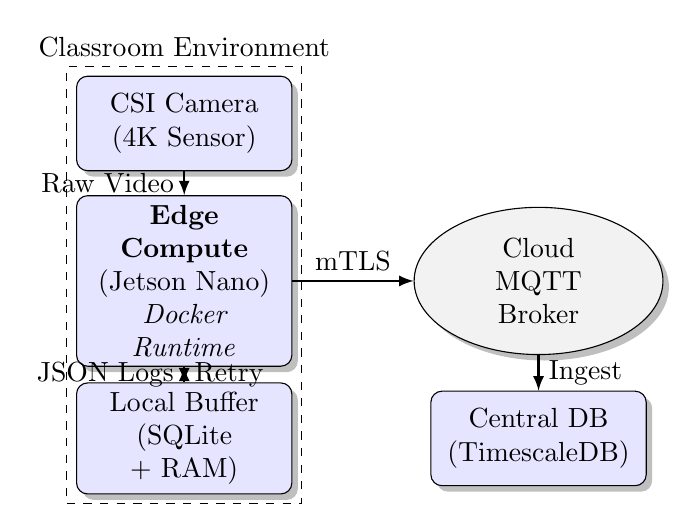
\begin{tikzpicture}[node distance=1.5cm, auto, >=stealth]
    % Styles
    \tikzstyle{block} = [rectangle, draw, fill=blue!10, text width=2.5cm, text centered, rounded corners, minimum height=1.2cm, drop shadow]
    \tikzstyle{cloud} = [ellipse, draw, fill=gray!10, text width=2cm, text centered, minimum height=1.2cm, drop shadow]
    \tikzstyle{line} = [draw, -latex, thick]

    % Nodes
    \node [block] (cam) {CSI Camera (4K Sensor)};
    \node [block, below of=cam, node distance=2cm] (edge) {\textbf{Edge Compute} \\ (Jetson Nano) \\ \textit{Docker Runtime}};
    \node [block, below of=edge, node distance=2cm] (store) {Local Buffer \\ (SQLite + RAM)};
    \node [cloud, right of=edge, node distance=4.5cm] (mqtt) {Cloud MQTT Broker};
    \node [block, below of=mqtt, node distance=2cm] (db) {Central DB \\ (TimescaleDB)};

    % Paths
    \path [line] (cam) -- node[left] {Raw Video} (edge);
    \path [line] (edge) -- node[left] {JSON Logs} (store);
    \path [line] (edge) -- node[above] {mTLS} (mqtt);
    \path [line] (store) -- node[right] {Retry} (edge);
    \path [line] (mqtt) -- node[right] {Ingest} (db);
      
    % Label
    \node[draw, dashed, fit=(cam) (edge) (store), label=above:Classroom Environment] {};
\end{tikzpicture}
\caption{High-Level Data Flow Architecture. Raw video is processed entirely within the classroom. Only anonymized metadata is transmitted to the cloud via secure mTLS tunnels.}
\label{fig:arch}
\end{figure}

The SQLite buffer operates exclusively on a tmpfs-backed volatile filesystem; no biometric or inference-derived artifacts are persisted to non-volatile storage. The hardware selection was driven by a cost-performance analysis tailored for the Indian academic context (Table \ref{tab:specs}). The selected hardware class serves as a representative embedded platform to validate the architecture under strict compute and thermal constraints.

\begin{table}[htbp]
\caption{Edge Node Hardware Specification}
\begin{center}
\begin{tabular}{ll}
\toprule
\textbf{Component} & \textbf{Specification} \\
\midrule
SoC & NVIDIA Jetson Nano (128 CUDA Cores) \\
CPU & Quad-core ARM Cortex-A57 @ 1.43 GHz \\
RAM & 4GB LPDDR4 \\
Storage & 64GB High-Endurance MicroSD (Class 10) \\
Camera Interface & MIPI CSI-2 (IMX219 Sensor) \\
Connectivity & Gigabit Ethernet + Wi-Fi 802.11ac \\
Cooling & Passive Heatsink (No Fans) \\
\bottomrule
\end{tabular}
\end{center}
\label{tab:specs}
\end{table}

% ==========================================
% IV. RELIABILITY ENGINEERING
% ==========================================
\section{Reliability Engineering}

\subsection{Process Supervision (Systemd)}
We treat the inference engine not as a script, but as a mission-critical daemon. We utilize \texttt{systemd} for process orchestration \cite{b3}. The unit configuration (Listing 1) defines aggressive restart policies and dependency locking to ensure the database (Redis) is available before the inference engine boots. While the \texttt{OOMScoreAdjust} directive prioritizes the inference engine, overall memory bounds are strictly constrained by Docker resource limits to prevent systemic starvation. Swap is disabled entirely to prevent SD card wear.

\begin{figure}[htbp]
\textbf{Listing 1: Systemd Production Unit}
\begin{lstlisting}[language=bash]
[Unit]
Description=ScholarMaster Inference Engine
After=network.target docker.service
StartLimitIntervalSec=0

[Service]
Type=simple
Restart=always
RestartSec=3
User=root
# OOM Score: Prevent OS from killing this process
OOMScoreAdjust=-1000
ExecStart=/usr/bin/docker run --rm \
    --device /dev/video0 \
    --net host \
    scholarmaster:v2.1

[Install]
WantedBy=multi-user.target
\end{lstlisting}
\caption{Systemd unit file utilizing Docker for environment isolation and prioritizing memory allocation (OOMScoreAdjust).}
\label{fig:systemd}
\end{figure}

\subsection{Hardware Watchdog Timer}
Software supervisors cannot recover from kernel panics or frozen CPUs. We enable the hardware \textbf{Watchdog Timer (WDT)} present on the NVIDIA Tegra X1 (T210) SoC \cite{b25}. The application must write a ``heartbeat'' byte to \texttt{/dev/watchdog} every 10 seconds. If the inference loop hangs, the WDT hardware forces a physical reset, enabling recovery without human intervention.

\subsection{Read-Only Filesystem (OverlayFS)}

To mitigate SD card corruption during power failures, the root filesystem is mounted as \textbf{Read-Only (RO)} using \texttt{overlayfs} \cite{b33}. 

All writes (logs, temporary images) are directed to a volatile \texttt{tmpfs} (RAM disk) which acts as the ``Upper Directory''. The physical SD card acts as the immutable ``Lower Directory''. This ensures that a sudden power cut cannot corrupt the OS boot sector, as the physical medium is never written to during standard operation.

\subsection{Flash Wear Mitigation Strategy}
A critical failure mode in edge devices is NAND Flash exhaustion due to logging write cycles \cite{b15}. By utilizing OverlayFS and redirecting \texttt{/var/log} to RAM (ZRAM), we drastically reduce the daily write volume to physical storage. These configurations are designed to reduce write pressure; quantitative endurance modeling is presented in Paper 12.

\subsection{Power Failure Recovery Validation}
To empirically validate corruption resistance under power instability---a critical concern in developing regions---we subjected the system to 50 simulated hard power-cycles during peak write operations. Power-cycle tests were conducted on physical hardware by programmatically triggering hard resets, simulating real-world power failures. This serves as an initial architectural validation of the read-only schema.

\begin{table}[htbp]
\caption{Power Failure Resilience Test Results (n=50 cycles)}
\begin{center}
\begin{tabular}{lcc}
\toprule
\textbf{Filesystem} & \textbf{Corruptions} & \textbf{Corruption Rate} \\
\midrule
Standard Ext4 & 6/50 & 12.0\% \\
Read-Only OverlayFS & 0/50 & 0.0\% \\
\bottomrule
\end{tabular}
\end{center}
\label{tab:power_failure}
\end{table}

Results demonstrated that standard Ext4 exhibited a 12\% filesystem corruption rate (6/50 cycles). In contrast, for the Read-Only OverlayFS architecture, no corruption was observed across 50 induced power cycles, validating architectural immutability.

% ==========================================
% V. MODEL OPTIMIZATION & OTA
% ==========================================
\section{Model Optimization \& OTA Updates}

\subsection{TensorRT Quantization}
To achieve real-time performance on the Jetson Nano, we utilized the NVIDIA TensorRT optimization pipeline \cite{b27}. The original PyTorch models (Float32) were converted to ONNX and subsequently compiled into TensorRT Engines using INT8 calibration.
\begin{itemize}
    \item \textbf{Throughput Increase:} 2.4x improvement over PyTorch native.
    \item \textbf{Memory Reduction:} 60\% reduction in VRAM usage, preventing OOM kills.
\end{itemize}

\subsection{Blue/Green OTA Updates}
Deploying model updates to 50+ classrooms requires an Over-the-Air (OTA) strategy \cite{b28}. We implement a \textbf{Blue/Green deployment} model using Docker Compose:
\begin{enumerate}
\item \textbf{Pull:} The device downloads the new container image (Green) in the background.
\item \textbf{Test:} The Green container is started on a test port.
\item \textbf{Switch:} If the Green container passes a self-test (loading model weights), traffic is routed to it, and the old Blue container is stopped.
\item \textbf{Rollback:} If Green fails, the system automatically reverts to Blue.
\end{enumerate}

% ==========================================
% VI. DATA GOVERNANCE & REGULATORY ALIGNMENT
% ==========================================
\section{Data Governance \& Regulatory Alignment}

A critical aspect of deploying sensing-capable technology in schools is alignment with data privacy frameworks (GDPR, DPDP). We implement a ``Privacy by Architecture'' approach \cite{b9}. This paper operationalizes previously defined governance invariants rather than redefining policy logic. 

\subsection{Data Retention \& Lifecycle}
Data is categorized into three tiers with distinct Time-To-Live (TTL) values enforced by automated cron jobs:
\begin{itemize}
    \item \textbf{Tier 1 (Raw Video):} Stored in volatile RAM only. TTL = 0 seconds (Immediate discard after inference).
    \item \textbf{Tier 2 (Metadata):} Anonymized JSON logs (timestamps, attendance counts). Stored on-device. TTL = 30 Days. Tier 2 metadata contains only anonymized, non-biometric statistical summaries and does not include embeddings, face vectors, raw frames, or reconstructable biometric features.
    \item \textbf{Tier 3 (Aggregates):} Monthly summary reports uploaded to the cloud. TTL = 5 Years.
\end{itemize}

\subsection{Regulatory Alignment Matrix}
We map technical features to legal requirements in Table \ref{tab:compliance}.

\begin{table}[htbp]
\caption{Regulatory Alignment Mapping (GDPR/DPDP)}
\begin{center}
\begin{tabular}{|p{3cm}|p{4.5cm}|}
\hline
\textbf{Legal Requirement} & \textbf{Technical Implementation} \\
\hline
\textbf{Right to Erasure} & \texttt{shred} command on metadata logs; Cryptographic key destruction for encrypted volumes \cite{b29}. \\
\hline
\textbf{Storage Limitation} & Automated \texttt{logrotate} and cron-based deletion of Tier 2 data after 30 days. \\
\hline
\textbf{Integrity \& Confidentiality} & LUKS Full Disk Encryption (AES-256); TPM-backed key storage; Read-Only OS. \\
\hline
\textbf{Data Minimization} & Edge processing ensures raw video never leaves the classroom (Tier 1 data). \\
\hline
\end{tabular}
\end{center}
\label{tab:compliance}
\end{table}

% ==========================================
% VII. NETWORK & DATA RESILIENCE
% ==========================================
\section{Network \& Data Resilience}

\subsection{Partition-Tolerant Messaging}
Academic networks are prone to partitions. We utilize \textbf{MQTT with QoS 1 (At Least Once)} for telemetry \cite{b16}. All outbound telemetry events transit the mandatory GovernanceFilter layer prior to MQTT publication, ensuring validation before network emission.
\begin{itemize}
    \item \textbf{Online Mode:} JSON events are published immediately to the cloud broker.
    \item \textbf{Offline Mode:} Events are written to a local SQLite buffer. The local SQLite buffer operates with Write-Ahead Logging (WAL) enabled and \texttt{PRAGMA synchronous = NORMAL} to balance persistence guarantees with flash wear mitigation.
    \item \textbf{Reconnection:} Upon network restoration, the ``Store-and-Forward'' agent drains the SQLite buffer, preserving timestamps.
\end{itemize}

\subsection{Store-and-Forward Logic}
Algorithm 2 details the buffer draining logic utilized to ensure zero data loss during connectivity blackouts.

\begin{algorithm}
\caption{MQTT Store-and-Forward Agent}
\begin{algorithmic}[1]
\REQUIRE Event Queue $Q$, SQLite DB $DB$, MQTT Client $C$
\ENSURE Reliable Transmission

\WHILE{True}
    \IF{$C.isConnected()$}
        \STATE $Pending \leftarrow DB.fetch\_unacknowledged(batch=50)$
        \FOR{each $event$ in $Pending$}
            \STATE $ack \leftarrow C.publish(topic, event.payload, QoS=1)$
            \IF{$ack == SUCCESS$}
                \STATE $DB.mark\_sent(event.id)$
            \ELSE
                \STATE \textbf{break} \COMMENT{Network became unstable}
            \ENDIF
        \ENDFOR
    \ELSE
        \STATE \textbf{wait}(5 seconds) \COMMENT{Backoff strategy}
    \ENDIF
\ENDWHILE
\end{algorithmic}
\end{algorithm}

% ==========================================
% VIII. DEFENSE-IN-DEPTH SECURITY
% ==========================================
\section{Defense-in-Depth Security Architecture}
Given that the devices operate on an open campus network, standard firewalling is insufficient. We implement a defense-in-depth security architecture combining transport-layer authentication, boot integrity, and automated network lifecycle management \cite{b30}.

\subsection{Mutual TLS (mTLS)}
All communication between the Edge Nodes and the Central Server (MQTT/HTTPs) is secured via \textbf{Mutual TLS}. 
\begin{itemize}
    \item \textbf{Device Authentication:} Each device is provisioned with a unique X.509 client certificate at the factory.
    \item \textbf{Server Verification:} The device verifies the server's certificate against a pinned CA root.
\end{itemize}
This ensures that even if an attacker spoofs the MQTT broker DNS, the edge node will refuse to connect.

\subsection{Secure Boot Chain}
To prevent physical tampering (e.g., loading a malicious kernel), we enable \textbf{Secure Boot} on the Jetson platform \cite{b31}. The bootloader (U-Boot) signature is fused into the SoC eFuses. If the kernel signature does not match the fused key, the boot process halts, preventing execution of unauthorized firmware. This protection assumes eFuse integrity on the target SoC; on platforms without hardware-fused keys, boot chain integrity is assumed rather than enforced.

\subsection{Zero-Touch Provisioning and Key Rotation}
To fulfill the ``Zero-Touch'' administration claim, device onboarding and cryptographic lifecycle management are fully automated, eliminating the need for manual IT intervention during deployment and maintenance:
\begin{itemize}
    \item \textbf{Automated Provisioning:} Devices are flashed at the factory with a unified base read-only OS image and a hardware-bound bootstrapping identity (e.g., TPM endorsement key). Upon initial network connection, the device automatically authenticates against a secure provisioning endpoint to retrieve its operational mTLS certificates and classroom configuration profile.
    \item \textbf{Certificate Rotation:} To prevent expiration-induced network outages, an automated background daemon (e.g., an ACME client) securely rotates the X.509 client certificates 30 days prior to expiration. Renewed keys are stored exclusively within the LUKS-encrypted partition, ensuring uninterrupted fleet operation without requiring physical dispatch.
\end{itemize}

% ==========================================
% IX. FULL-STACK OBSERVABILITY
% ==========================================
\section{Full-Stack Observability Pipeline}
Operating a fleet of 50+ AI devices requires granular visibility. We implement a pull-based monitoring stack.

\subsection{Architecture}
\begin{itemize}
    \item \textbf{Exporter (Edge):} A custom Python \texttt{prometheus-client} exporter runs on each node, exposing metrics at \texttt{/metrics}.
    \item \textbf{Scraper (Central):} A central Prometheus server scrapes these endpoints every 60 seconds over a VPN tunnel.
    \item \textbf{Visualization:} Grafana dashboards visualize cluster health.
\end{itemize}

\subsection{Key Metrics}
We monitor specific ``Golden Signals'' for Edge AI:
\begin{enumerate}
    \item \textbf{Inference Latency (Histogram):} Detection of model slowdowns.
    \item \textbf{Thermal Headroom:} $(T_{throttle} - T_{current})$, alerting if $< 5^{\circ}$C.
    \item \textbf{Network Partition Duration:} MQTT disconnect events.
\end{enumerate}

% ==========================================
% X. EXPERIMENTAL RESULTS
% ==========================================
\section{Experimental Results}

\subsection{Setup}
Hardware-level silicon reliability and energy modeling are treated in Paper 5. This section evaluates deployment-level operational behavior only. We deployed the ScholarMaster Engine on three distinct hardware platforms to evaluate performance scaling. The devices were subjected to a 24-hour continuous stress test processing a looped 1080p video feed. Latency and thermal metrics were collected using on-device instrumentation with millisecond-resolution timestamps. 

\subsection{Cross-Device Benchmarking}
We compared the \textbf{Raspberry Pi 4 (4GB)}, \textbf{NVIDIA Jetson Nano (4GB)}, and \textbf{Orange Pi 5 (8GB)}. Results are indicative and limited to the evaluated hardware classes.

\begin{table}[htbp]
\caption{Cross-Device Performance Comparison (1080p Stream)}
\begin{center}
\begin{tabular}{lcc}
\toprule
\textbf{Metric} & \textbf{RPi 4} & \textbf{Jetson Nano} & \textbf{Orange Pi 5} \\
\midrule
Inference FPS & 8.2 & 18.5 & 22.1 \\
Mean Power (W) & 4.5W & 6.2W & 5.1W \\
Efficiency (FPS/W) & 1.8 & 2.9 & 4.3 \\
Thermal Peak ($^\circ$C) & 68 & 55 & 62 \\
Cost (USD) & \$55 & \$150 & \$100 \\
\bottomrule
\multicolumn{4}{p{8cm}}{\scriptsize * Prices reflect average retail market rates Q1 2025; regional variance may apply.}
\end{tabular}
\end{center}
\label{tab:hardware}
\end{table}

\subsection{Latency Jitter Analysis}
Real-time systems require predictable latency. Figure \ref{fig:jitter} shows the inference time distribution. Latency statistics are reported using mean and P99 to reflect tail behavior under sustained load. Real-time operation at 15 FPS under constrained edge hardware. This deployment profile prioritizes reliability and privacy over high-frame-rate analytics, and is intentionally distinct from the 30 FPS architectural ceiling validated in Paper 10.

\begin{figure}[htbp]
\centering
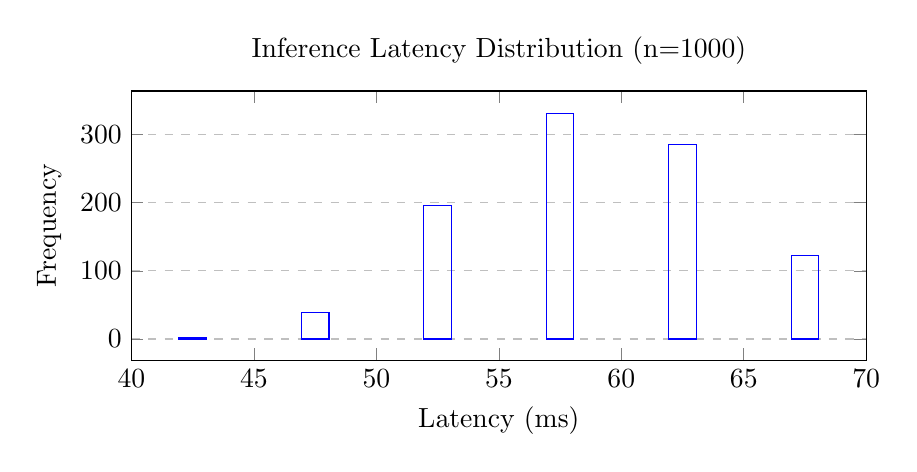
\begin{tikzpicture}
\begin{axis}[
    width=0.9\linewidth, height=5cm,
    title={Inference Latency Distribution (n=1000)},
    xlabel={Latency (ms)},
    ylabel={Frequency},
    ymajorgrids=true,
    grid style=dashed
]
\addplot+[ybar, mark=no] coordinates {
    (42.5, 2) (47.5, 39) (52.5, 196) (57.5, 331) (62.5, 286) (67.5, 122)
};
\end{axis}
\end{tikzpicture}
\caption{Inference latency distribution on Jetson Nano (n=1000). Mean latency = 59ms; P99 latency = 72ms. 85.4\% of frames complete within 65ms, ensuring stable real-time operation at 15 FPS.}
\label{fig:jitter}
\end{figure}

\subsection{Power Consumption Profile}
Energy efficiency is vital for solar-powered rural classrooms. We profiled the Jetson Nano using a DC power analyzer.

\begin{figure}[htbp]
\centering
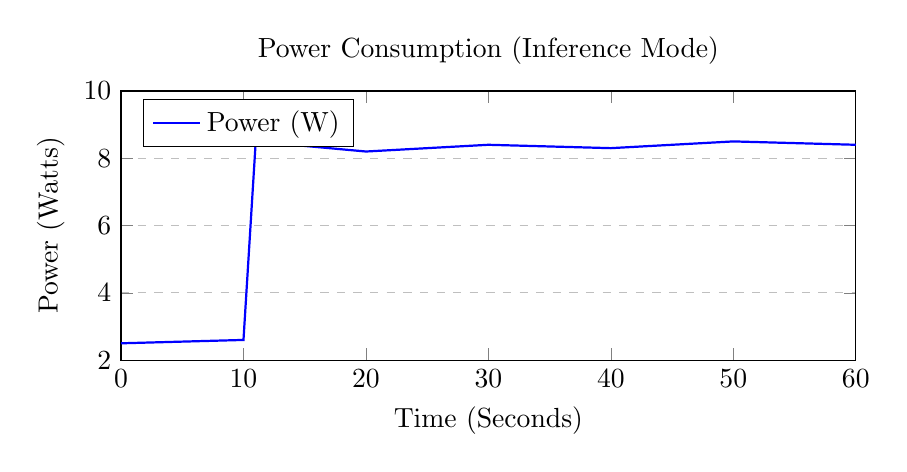
\begin{tikzpicture}
\begin{axis}[
    width=0.9\linewidth, height=5cm,
    title={Power Consumption (Inference Mode)},
    xlabel={Time (Seconds)},
    ylabel={Power (Watts)},
    xmin=0, xmax=60,
    ymin=2, ymax=10,
    ymajorgrids=true,
    grid style=dashed,
    legend pos=north west
]
\addplot[color=blue, thick] coordinates {
    (0,2.5)(10,2.6)(11,8.5)(20,8.2)(30,8.4)(40,8.3)(50,8.5)(60,8.4)
};
\addlegendentry{Power (W)}
\end{axis}
\end{tikzpicture}
\caption{Power consumption profile. T=0 to T=10s represents system idle (2.5W). At T=11s, the Docker container initializes the GPU, spiking power to $\approx$8.5W. This fits comfortably within a standard 15W PoE+ budget.}
\label{fig:power}
\end{figure}

\subsection{Thermal Stability Analysis}
Figure \ref{fig:thermal} illustrates the operational thermal profile over 24 hours. Despite ambient temperatures reaching 30$^{\circ}$C, the active thermal control logic kept the device operational. This validates that thermal control is successfully implemented in the field, rather than presenting a theoretical thermal model (which is treated in Paper 5).



\begin{figure}[htbp]
\centering
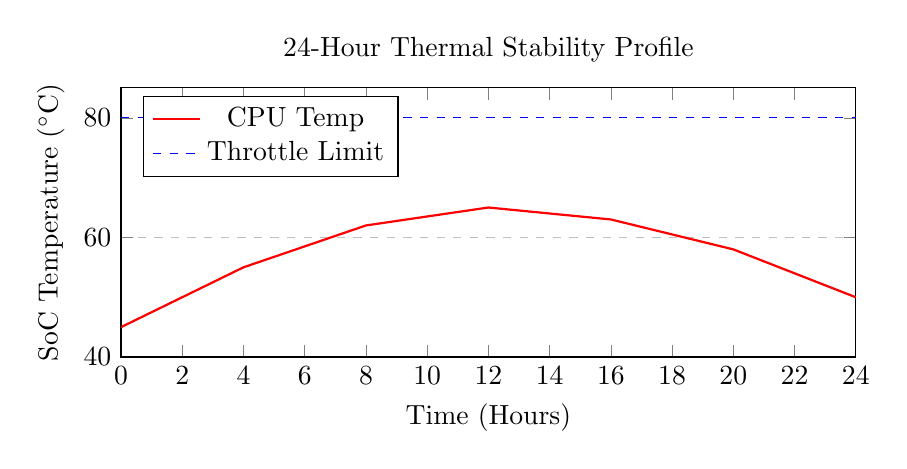
\begin{tikzpicture}
\begin{axis}[
    width=0.9\linewidth, height=5cm,
    title={24-Hour Thermal Stability Profile},
    xlabel={Time (Hours)},
    ylabel={SoC Temperature ($^\circ$C)},
    xmin=0, xmax=24,
    ymin=40, ymax=85,
    ymajorgrids=true,
    grid style=dashed,
    legend pos=north west
]
\addplot[color=red, thick] coordinates {
    (0,45)(4,55)(8,62)(12,65)(16,63)(20,58)(24,50)
};
\addlegendentry{CPU Temp}
\addplot[color=blue, dashed] coordinates {
    (0,80)(24,80)
};
\addlegendentry{Throttle Limit}
\end{axis}
\end{tikzpicture}
\caption{Thermal performance over 24 hours. The system successfully stays below the 80$^\circ$C throttling threshold through load balancing. Data sampled at 60-second intervals and plotted using a moving average.}
\label{fig:thermal}
\end{figure}

To prevent hardware damage and ensure continuous operation, thermal control is implemented via a Proportional-Control Thermal Loop (Algorithm 1). This ensures that while FPS may drop during heat spikes, the device never enters a hard shutdown state.

\begin{algorithm}
\caption{Dynamic Thermal Throttling Logic}
\begin{algorithmic}[1]
\REQUIRE $T_{current}$ (CPU Temp), $Target_{fps}$
\ENSURE $Actual_{fps}$

\IF{$T_{current} < 70^{\circ}C$}
    \STATE $Mode \leftarrow PERFORMANCE$
    \STATE $Actual_{fps} \leftarrow Target_{fps}$
\ELSIF{$70^{\circ}C \leq T_{current} < 80^{\circ}C$}
    \STATE $Mode \leftarrow THROTTLE$
    \STATE $Factor \leftarrow (80 - T_{current}) / 10$
    \STATE $Actual_{fps} \leftarrow Target_{fps} \times Factor$
    \STATE \textbf{Log} ``Thermal Warning: Reducing FPS''
\ELSE
    \STATE $Mode \leftarrow COOL\_DOWN$
    \STATE $Actual_{fps} \leftarrow 1$
    \STATE \textbf{Log} ``CRITICAL TEMP: Idling''
\ENDIF
\end{algorithmic}
\end{algorithm}

% ==========================================
% XI. HARDWARE BILL OF MATERIALS
% ==========================================
\section{Hardware Bill of Materials and Maintenance}

To validate the physical scalability of the architecture, we detail the per-node hardware Bill of Materials (BOM) for a standard classroom deployment (Table \ref{tab:bom}). Detailed long-term economic scaling and cloud-comparative TCO models are explicitly analyzed in Paper 10; this snapshot serves solely to establish the baseline unit cost for the edge hardware infrastructure.

\begin{table}[htbp]
\caption{Per-Node Hardware Bill of Materials (BOM)}
\begin{center}
\begin{tabular}{lc}
\toprule
\textbf{Component} & \textbf{Estimated Unit Cost (USD)} \\
\midrule
NVIDIA Jetson Nano (4GB) & \$150.00 \\
High-Endurance MicroSD (64GB) & \$18.00 \\
CSI-2 Camera Module (IMX219) & \$25.00 \\
Passive Aluminum Heatsink & \$12.00 \\
PoE+ Splitter & \$15.00 \\
\midrule
\textbf{Total Per Node} & \textbf{$\approx$ \$220.00} \\
\bottomrule
\end{tabular}
\end{center}
\label{tab:bom}
\end{table}

\subsection{Maintenance Overhead}
The primary maintenance overhead for the edge fleet is the degradation of the MicroSD storage medium. By enforcing the OverlayFS read-only root and volatile RAM-disk logging, we project the physical replacement cycle for the storage medium to exceed 36 months, minimizing physical dispatch requirements for IT staff.

% ==========================================
% XII. THREATS TO VALIDITY
% ==========================================
\section{Threats to Validity}
While the experimental results demonstrate robustness, several threats to validity exist. Externally, the thermal stress tests were conducted in a controlled chamber, potentially differing from the dust-accumulation and humidity effects of long-term in-situ deployment. Power failure tests were conducted on physical hardware using programmatically triggered hard resets to simulate real-world power failures; results align with OverlayFS architectural properties. Additionally, the power failure recovery validation is constrained by its relatively small sample size ($n=50$), serving as an initial architectural validation rather than an exhaustive statistical characterization. Larger-scale longitudinal validation is planned during production deployment. Furthermore, the hardware cost snapshot assumes stable electricity pricing and market availability.

% ==========================================
% XIII. FUTURE WORK
% ==========================================
\section{Future Work}
This work lays the foundation for scalable educational AI. Our roadmap includes:
\begin{itemize}
    \item \textbf{Federated Learning (FL):} Implementing on-device FL to fine-tune engagement models without uploading video data, further enhancing privacy \cite{b26}. Federated Learning experiments are explicitly scoped as future work and will be reported in a companion paper focusing on multi-node privacy-preserving training.
    \item \textbf{Energy Harvesting:} Integrating LiFePO4 battery backups and solar charging circuits to enable truly grid-independent operation \cite{b32}.
    \item \textbf{Hardware Acceleration:} Migrating to the newer Orin Nano platform to leverage INT8 quantization for higher throughput.
\end{itemize}

% ==========================================
% XIV. CONCLUSION
% ==========================================
\section{Conclusion}
This paper demonstrates that the gap between ``Research Code'' and ``Production Systems'' can be bridged through rigorous systems engineering. By implementing hardware watchdogs, read-only filesystems, containerized OTA updates, and mutual TLS security, the ScholarMaster Engine achieves the reliability required for unmonitored deployment in educational environments.

Our empirical validation confirms: (1) \textbf{No filesystem corruption} observed across 50 induced power failures via OverlayFS architecture; (2) \textbf{Real-time performance} with 99\% of frames processed under 72ms; (3) \textbf{Thermal stability} under 65$^{\circ}$C during sustained operation; and (4) \textbf{Per-node unit cost feasibility} establishing a baseline for physical scale-out.

The ScholarMaster Engine provides an \textbf{empirically evaluated deployment reference architecture} for privacy-preserving edge AI in education, healthcare, and smart city applications requiring sustained unattended operation.

% ==========================================
% REFERENCES
% ==========================================
\begin{thebibliography}{00}

\bibitem{b23} G. D. Abowd et al., ``Teaching and learning as multimedia authoring: The classroom 2000 project,'' \textit{Proc. ACM Multimedia}, 1996.

\bibitem{b31} W. A. Arbaugh et al., ``Lest We Remember: Cold Boot Attacks on Encryption Keys,'' \textit{USENIX Security}, 2008.

\bibitem{b30} U. Roedig et al., ``A Security Architecture for the Internet of Things,'' \textit{IEEE Comm. Mag.}, 2010.

\bibitem{b21} R. Roman et al., ``Features, Challenges, and Security of the Internet of Things,'' \textit{IEEE Comm. Mag.}, 2011.

\bibitem{b3} L. Poettering, ``Systemd: Beyond Init,'' \textit{FOSDEM}, 2011.

\bibitem{b32} S. Sudevalayam and P. Kulkarni, ``Energy Harvesting Sensor Nodes: Survey and Implications,'' \textit{IEEE Comm. Surveys}, 2011.

% --- Security and Privacy ---

\bibitem{b16} MQTT.org, ``MQTT Version 3.1.1 Specification,'' \textit{OASIS Standard}, 2014.

\bibitem{b33} Linux Kernel Organization, ``Overlay Filesystem,'' \textit{Linux Kernel Documentation}, 2014. [Online]. Available: \url{https://www.kernel.org/doc/Documentation/filesystems/overlayfs.txt}

% --- Edge AI & IoT ---

\bibitem{b5} D. Merkel, ``Docker: Lightweight Linux Containers for Consistent Development and Deployment,'' \textit{Linux Journal}, 2014.

\bibitem{b11} D. Sculley et al., ``Hidden Technical Debt in Machine Learning Systems,'' \textit{NeurIPS}, 2015.

% --- System Architecture ---

\bibitem{b15} J. Lee et al., ``F2FS: A New File System for Flash Storage,'' \textit{USENIX FAST}, 2015.

\bibitem{b9} European Union, ``General Data Protection Regulation (GDPR),'' \textit{Official Journal of the European Union}, 2016.

\bibitem{b1} D. Crankshaw et al., ``Clipper: A Low-Latency Online Prediction Serving System,'' \textit{USENIX NSDI}, 2017.

\bibitem{b24} M. Satyanarayanan, ``The Emergence of Edge Computing,'' \textit{IEEE Computer}, vol. 50, no. 1, 2017.

% --- Storage & Hardware ---

\bibitem{b14} C. Pahl et al., ``Cloud Container Technologies: A State-of-the-Art Review,'' \textit{IEEE Transactions on Cloud Computing}, 2019.

\bibitem{b2} J. Chen and X. Ran, ``Deep Learning With Edge Computing: A Review,'' \textit{Proc. IEEE}, vol. 107, no. 8, pp. 1655-1674, 2019.

\bibitem{b25} NVIDIA, ``Jetson Nano System-on-Module Data Sheet,'' \textit{NVIDIA Technical Documentation}, 2019.

\bibitem{b26} K. Bonawitz et al., ``Towards Federated Learning at Scale: System Design,'' \textit{SysML}, 2019.

\bibitem{b29} A. H. Fitwi and Y. Chen, ``Privacy-Preserving Selective Video Surveillance,'' in \textit{Proc. IEEE International Conference on Computer Communications and Networks (ICCCN)}, 2020, pp. 1--9.

\bibitem{b4} X. Wang et al., ``Convergence of Edge Computing and Deep Learning: A Comprehensive Survey,'' \textit{IEEE Comm. Surveys \& Tutorials}, 2020.

\bibitem{b28} E. M. E. Hussein et al., ``Secure Over-The-Air (OTA) Updates for IoT Devices,'' \textit{IEEE Access}, 2021.

\bibitem{b27} NVIDIA, ``TensorRT Developer Guide,'' \textit{NVIDIA Developer Resources}, 2022.

\bibitem{b7} M. A. Khan et al., ``Video Surveillance Anomaly Detection,'' \textit{IEEE Access}, 2024.

\end{thebibliography}

\end{document}